

%=======================   Default Templete   ==================
\documentclass[11pt]{article}
\usepackage{graphicx}

% file with some default definations
%%%%%%%%%%%%%%%%%%%%%%%%%%%%%%%%%%%%%%%%%
% Lachaise Assignment
% Structure Specification File
% Version 1.0 (26/6/2018)
%
% This template originates from:
% http://www.LaTeXTemplates.com
%
% Authors:
% Marion Lachaise & François Févotte
% Vel (vel@LaTeXTemplates.com)
%
% License:
% CC BY-NC-SA 3.0 (http://creativecommons.org/licenses/by-nc-sa/3.0/)
% 
%%%%%%%%%%%%%%%%%%%%%%%%%%%%%%%%%%%%%%%%%

%----------------------------------------------------------------------------------------
%	PACKAGES AND OTHER DOCUMENT CONFIGURATIONS
%----------------------------------------------------------------------------------------

\usepackage{amsmath,amsfonts,stmaryrd,amssymb} % Math packages

\usepackage{amsthm}

\usepackage{enumerate} % Custom item numbers for enumerations

\usepackage[ruled]{algorithm2e} % Algorithms

\usepackage[framemethod=tikz]{mdframed} % Allows defining custom boxed/framed environments

\usepackage{listings} % File listings, with syntax highlighting
\lstset{
	basicstyle=\ttfamily, % Typeset listings in monospace font
}

%----------------------------------------------------------------------------------------
%	DOCUMENT MARGINS
%----------------------------------------------------------------------------------------

\usepackage{geometry} % Required for adjusting page dimensions and margins

\geometry{
	paper=a4paper, % Paper size, change to letterpaper for US letter size
	top=2.5cm, % Top margin
	bottom=3cm, % Bottom margin
	left=2.5cm, % Left margin
	right=2.5cm, % Right margin
	headheight=14pt, % Header height
	footskip=1.5cm, % Space from the bottom margin to the baseline of the footer
	headsep=1.2cm, % Space from the top margin to the baseline of the header
	%showframe, % Uncomment to show how the type block is set on the page
}

%----------------------------------------------------------------------------------------
%	FONTS
%----------------------------------------------------------------------------------------

\usepackage[utf8]{inputenc} % Required for inputting international characters
\usepackage[T1]{fontenc} % Output font encoding for international characters

\usepackage{XCharter} % Use the XCharter fonts

%----------------------------------------------------------------------------------------
%	COMMAND LINE ENVIRONMENT
%----------------------------------------------------------------------------------------

% Usage:
% \begin{commandline}
%	\begin{verbatim}
%		$ ls
%		
%		Applications	Desktop	...
%	\end{verbatim}
% \end{commandline}

\mdfdefinestyle{commandline}{
	leftmargin=10pt,
	rightmargin=10pt,
	innerleftmargin=15pt,
	middlelinecolor=black!50!white,
	middlelinewidth=2pt,
	frametitlerule=false,
	backgroundcolor=black!5!white,
	frametitle={Command Line},
	frametitlefont={\normalfont\sffamily\color{white}\hspace{-1em}},
	frametitlebackgroundcolor=black!50!white,
	nobreak,
}

% Define a custom environment for command-line snapshots
\newenvironment{commandline}{
	\medskip
	\begin{mdframed}[style=commandline]
}{
	\end{mdframed}
	\medskip
}

%----------------------------------------------------------------------------------------
%	FILE CONTENTS ENVIRONMENT
%----------------------------------------------------------------------------------------

% Usage:
% \begin{file}[optional filename, defaults to "File"]
%	File contents, for example, with a listings environment
% \end{file}

\mdfdefinestyle{file}{
	innertopmargin=1.6\baselineskip,
	innerbottommargin=0.8\baselineskip,
	topline=false, bottomline=false,
	leftline=false, rightline=false,
	leftmargin=2cm,
	rightmargin=2cm,
	singleextra={%
		\draw[fill=black!10!white](P)++(0,-1.2em)rectangle(P-|O);
		\node[anchor=north west]
		at(P-|O){\ttfamily\mdfilename};
		%
		\def\l{3em}
		\draw(O-|P)++(-\l,0)--++(\l,\l)--(P)--(P-|O)--(O)--cycle;
		\draw(O-|P)++(-\l,0)--++(0,\l)--++(\l,0);
	},
	nobreak,
}

% Define a custom environment for file contents
\newenvironment{file}[1][File]{ % Set the default filename to "File"
	\medskip
	\newcommand{\mdfilename}{#1}
	\begin{mdframed}[style=file]
}{
	\end{mdframed}
	\medskip
}

%----------------------------------------------------------------------------------------
%	NUMBERED QUESTIONS ENVIRONMENT
%----------------------------------------------------------------------------------------

% Usage:
% \begin{question}[optional title]
%	Question contents
% \end{question}

\mdfdefinestyle{question}{
	innertopmargin=1.2\baselineskip,
	innerbottommargin=0.8\baselineskip,
	roundcorner=5pt,
	nobreak,
	singleextra={%
		\draw(P-|O)node[xshift=1em,anchor=west,fill=white,draw,rounded corners=5pt]{%
		Question \theQuestion\questionTitle};
	},
}

\newcounter{Question} % Stores the current question number that gets iterated with each new question

% Define a custom environment for numbered questions
\newenvironment{question}[1][\unskip]{
	\bigskip
	\stepcounter{Question}
	\newcommand{\questionTitle}{~#1}
	\begin{mdframed}[style=question]
}{
	\end{mdframed}
	\medskip
}

%----------------------------------------------------------------------------------------
%	WARNING TEXT ENVIRONMENT
%----------------------------------------------------------------------------------------

% Usage:
% \begin{warn}[optional title, defaults to "Warning:"]
%	Contents
% \end{warn}

\mdfdefinestyle{warning}{
	topline=false, bottomline=false,
	leftline=false, rightline=false,
	nobreak,
	singleextra={%
		\draw(P-|O)++(-0.5em,0)node(tmp1){};
		\draw(P-|O)++(0.5em,0)node(tmp2){};
		\fill[black,rotate around={45:(P-|O)}](tmp1)rectangle(tmp2);
		\node at(P-|O){\color{white}\scriptsize\bf !};
		\draw[very thick](P-|O)++(0,-1em)--(O);%--(O-|P);
	}
}

% Define a custom environment for warning text
\newenvironment{warn}[1][Warning:]{ % Set the default warning to "Warning:"
	\medskip
	\begin{mdframed}[style=warning]
		\noindent{\textbf{#1}}
}{
	\end{mdframed}
}

%----------------------------------------------------------------------------------------
%	INFORMATION ENVIRONMENT
%----------------------------------------------------------------------------------------

% Usage:
% \begin{info}[optional title, defaults to "Info:"]
% 	contents
% 	\end{info}

\mdfdefinestyle{info}{%
	topline=false, bottomline=false,
	leftline=false, rightline=false,
	nobreak,
	singleextra={%
		\fill[black](P-|O)circle[radius=0.4em];
		\node at(P-|O){\color{white}\scriptsize\bf i};
		\draw[very thick](P-|O)++(0,-0.8em)--(O);%--(O-|P);
	}
}

% Define a custom environment for information
\newenvironment{info}[1][Info:]{ % Set the default title to "Info:"
	\medskip
	\begin{mdframed}[style=info]
		\noindent{\textbf{#1}}
}{
	\end{mdframed}
}
\usepackage{listings}
\lstset{language=Bash, basicstyle=\normalsize\linespread{0.8}, stepnumber=1, numbersep=5pt}
\usepackage{fancyhdr}
\usepackage{pdfpages} 
\setlength{\parindent}{0pt}
\fancypagestyle{note_1}{\fancyfoot[R]{\textit{* These kind of auction are sealed bid auction.}}}
\pagestyle{fancy}
\fancyhf{}
\lhead{\textit{Auto Scaling of Key Value stores}}
\chead{\textit{UGP Report}}
\rhead{\COURSE}
\usepackage{cite}

%==================Header details======================
\newcommand\NAME{Raghukul Raman}
\newcommand\ANDREWID{160538}
\newcommand\HWNUM{4}
\newcommand\COURSE{CS396}
%======================================================

% available formatted sections:
% - COMMAND LINE ENVIRONMENT: \begin{commandline} \end{commandline}
% - FILE CONTENTS ENVIRONMENT: \begin{file}[optional filename, defaults to "File"]
% - NUMBERED QUESTIONS ENVIRONMENT: \begin{question}[optional title]
% - WARNING TEXT ENVIRONMENT(can also be used for note): \begin{warn}[optional title, defaults to "Warning:"]
% - INFORMATION ENVIRONMENT(can be used to mention given details): \begin{info}[optional title, defaults to "Info:"]

%===============================================================
\begin{document}
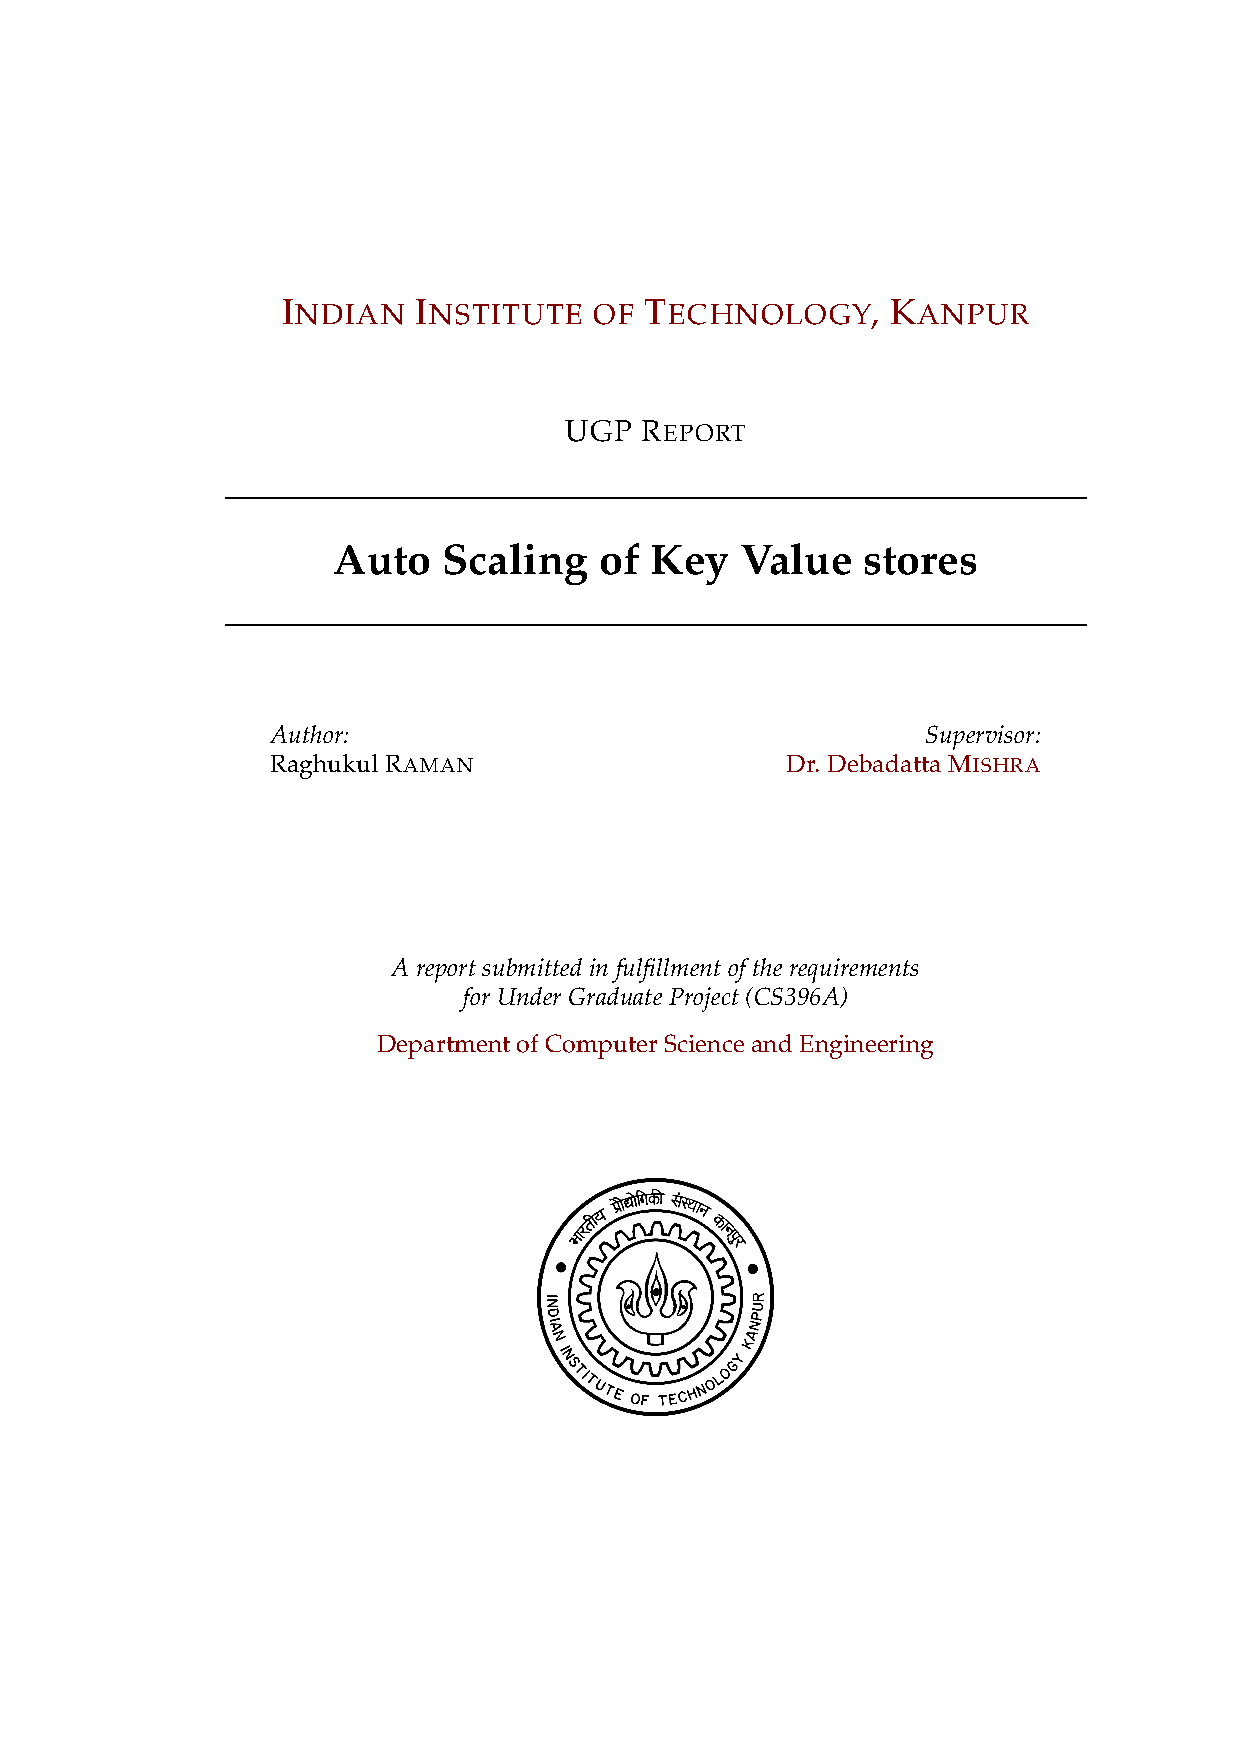
\includepdf[page={1}]{first_page.pdf}
\section*{Abstract}
In the modern day computing where application response is a 
critical metric, in memory databases are gaining popularity. In-memory 
databases primarily use main memory for data storage. These databases 
are becoming a crucial part of many applications due to the availability 
of less expensive RAM, and the demand for high response time.  Some of 
the cases where in-memory databases perform exceptionally well are 
Queues, sticky sessions, caching, real-time data analysis, etc.
\\

Generally, these in-memory databases are implemented as key-value 
stores; some well know key-value stores are Redis, Memcached, Hazelcast, 
etc. Large scale caching can be done by scaling the instances of these 
databases. Dynamic scaling of instances can provide cost-effective 
key-value storage services.This project aims at analyzing and providing 
an auto-scaling solution to this problem.
\\

We try to collect statistics for different queries on different node 
configurations and try to find possible bottlenecks in the cluster based 
system. We analyze by scaling redis horizontally as well as vertically. 
For analyzing clusters we use an open source tool called Twemproxy (a 
fast, light-weight proxy for Memcached and redis). We limit resources 
and measure performance for these configurations. We also try to build a 
system which can be used to interact with the cluster and efficiently 
shard the requests among different instances.




% In the modern world where application response is a critical metric,
% in memory databases are gaining wide popularity. In-memory databases primarily relies
% on main memory for data storage. These databases are becoming a crucial part of many
% applications due to the availability of less expensive RAM, and the demand for high response time.
% Accessing data in memory eliminates seek time when querying the data,
% which provides faster and more predictable performance than disk.
% Some of the cases where in-memory databases perform exceptionally well are Queues,
% sticky sessions, caching, real-time analysis of data, etc. \\
% 
% Generally, these in-memory databases are implemented as key-value stores;
% some traditional ones are Redis, Memcached, Hazelcast, etc. Large scale caching
% can be done by scaling the instances of these databases. One way is running a fixed number of instances,
% while the other is to scale up/down based on the load that our sever gets.
% This project aims at analyzing and providing an auto-scaling solution to this problem. \\
% 
% First, we try to collect statistics for different queries on different node
% configurations and try to find possible bottlenecks in the cluster based system.
% We analyze by scaling redis horizontally as well as vertically and try to explain the results.
% For analyzing clusters we use an open source tool called Twemproxy
% (a fast, light-weight proxy for Memcached and redis). We try to limit resources and
% measure performance for these configurations. We also try to build a system which can
% be used to interact with the cluster and efficiently shard the requests among
% different instances. Second part of the project is to give a scaling algorithm based on machine learning
% and some statistical predictions.




\pagebreak
\section*{Introduction}
\subsection*{Key Value Stores}
Key value stores are a special kind of database management system, where the 
data is organized in just $2$ columns - a key, and a value. Here the key is mostly
text, while the value can be anything and is simply an object. The actual data
essentially becomes "value", which is indexed with "key", so whole data 
becomes schema-less and is just organized in just $2$ columns. One important property
is that since the data is indexed by just the keys, there is a lot of scope of
distributing keys over different instances, making the system highly scalable.
\\

These kind of databases fall into the category of nosql data stores, satisfying the 
BASE properties (Basically Available, Soft state, Eventually consistent).
In the contezt of the CAP theorem (Consistency, Availability, Partition tolerance), these
databases fall into the category of CP. Since these databases are generally implemented
in cluster mode, we cannot gurantee availability on data.
\\

These databases are generally in-memory which reside in main memory. In-memory
databases are faster than disk-optimized databases because disk access is 
slower than memory access, the internal optimization algorithms 
are simpler and execute fewer CPU instructions.

\subsection*{Scalability}
\textbf{Scalability} is the property of a system to handle a growing amount of work
by adding resources to the system \cite{scaling}. In layman terms, when
you realise your system is getting slow and is unable to handle
the current number of requests, you need to scale the system. Scaling 
can be done in two ways:

\begin{itemize}
    \item \textbf{Vertical Scaling:} Increasing the resources in the server
            which we are currently using, i.e increase the amount of CPU, GPU,
            CPU, etc. Vertical scaling generally costly, also it may
            require the system to go down for a moment when the scaling takes
            place (need for downtime).
    \item \textbf{Horizontal Scaling:} Increasing the number of servers (instances).
            This would lead to decrease in the overall load on the system, if requests
            are sharded properly. This kind of scaling solution is typically popular 
            in tech industries, as it makes the system fault tolerant (single point of
            failure reduced). Important advantage of this method is that it can provide
            administrators with the ability to increase capacity on the fly.
\end{itemize}

\subsection*{Redis}
Redis project started by Salvatore Sanfilippo(\textit{antirez}) is
an open source, in-memory data structure store,
used as a database, cache and message broker \cite{redis}.
Apart from basic key-value structure it also supports other data structures like:
strings, hashes, lists, sets, sorted sets with range queries, bitmaps,
hyperloglogs, geospatial indexes with radius queries and streams. Redis has built in
support for replication, on-disk persistance and automated partitioning with Redis cluster.
Redis also supports trivial-to-setup master-slave asynchronous
replication, with very fast non-blocking first synchronization, auto-reconnection
with partial resynchronization on net split \cite{redis}.
There is also support to run these operations in atomic fashion with the help
of transactions.
\\

One intruging property of redis which makes it different from other classical key
value stores is: it gives support to mention expiration time for keys. This features
comes handy when we are using redis for cache purpose, olders keys would be deleted automatically.

\pagebreak

\subsection*{Redis Cluster}
Redis cluster can be defined as a collection of redis nodes which are able to communicate
among themselves, and are able to respond to requests collectively.
Redis Cluster provides a way to run a Redis installation where
data is automatically sharded across multiple Redis nodes.
Redis Cluster also provides some degree of availability during partitions
that is in practical terms the ability to continue the operations when
some nodes fail or are not able to communicate \cite{redis}.
\\

Every redis cluster node require two TCP ports, the lower one is used to server clients,
while the higher one(lower port+10000) is used for Cluster bus (node-to-node communication).
Redis cluster use CRC16 hashing system, using which every key is hashed to
becomes part of one of $16384$ hash slots (these are like buckets 
which contain keys, after hashing). So each cluster node is
responsible for a subset of hash slots, that is keys which hash to a particluar
hash slot, would be found in the node serving that hash slot.
The user can force multiple keys to be part of the same hash slot
by using a concept called hash tags.


\subsubsection*{Creating a Redis Cluster}
To create a redis cluster we need to run the required number of instances of redis
(on different ports), and then inform all these nodes about cluster meet. A typical
redis config file for cluster node is:
\begin{file}[redis.conf]
port $6379$ \\
cluster-enabled yes \\
cluster-config-file nodes.conf \\
cluster-node-timeout $5000$ \\
appendonly yes \\
\end{file}

After running all the required number of instances(with different ports, if
running on same machine), we need to run:
\begin{lstlisting}
$ redis-cli --cluster create 127.0.0.1:7000 127.0.0.1:7001 \
127.0.0.1:7002 127.0.0.1:7003 127.0.0.1:7004 127.0.0.1:7005 
\end{lstlisting}
Here the IPs mentioned are the host and ports of the redis instances. After 
running this command we are asked about the hash slot distribution, to be configured
among the nodes. And that's it, all the node share infomation about cluster,
and other nodes via messaging protocol. So after this process, each node will have a
hash slot to node (IP:PORT) mapping, and all other cluster informations like node timeout etc.

\subsubsection*{Redirection and Resharding}
We assume that a client know nothing about the distribution of hash slots in the cluster,
so it is equally probable to send a request to any of the node.
On recieving a request, the redis node will find the hash slot to which this key
belongs, if the hash slot is served by current node, it would simply return the value
to the client. Is case hash slot is not served, it would check its internal hash slot
to node map, and would respond to the client with an MOVED error, along this error
message it would also send the IP of the node serving hash slot to which this key maps.
This is pretty handy since client doesn't have to hit and try every node,
it would get the correct address after one try. Still there is an overhead, since we
need to send a request twice (in worst case). We'll come to this issue in more detail
in the partitioning section.
\\

Redis Cluster supports the ability to add and remove nodes while the
cluster is running. Adding or removing a node is abstracted into
the same operation: moving a hash slot from one node to another. This
means that the same basic mechanism can be used in order to rebalance the
cluster, add or remove nodes, and so forth. Moving slots in running cluster 
is not an issue, since if the hash key is present in current node, it would simply 
return the value, in case that particular key is moved to another node, it would
respond with an moved error. Hence resharding can we done in redis cluster without
any down time.

\subsubsection*{Partioning}
Partioning refers to the way how we shard data among
different nodes of redis cluster. Note that redis cluster provide a 
sharding scheme based on CRC16, but we can make some custom modification in the sharding
scheme at different levels, these are:
\begin{enumerate}
    \item \textbf{Client side partitioning}: In this scheme, redis clients select the
        node to which read/write request need to be made.
    \item \textbf{Proxy assisted partitioning}: This scheme suggests that client sends
        request to a proxy, which analyzes the request and forwards it to the correct node.
        On recieving response it then returns it to the client. eg: Twemproxy
    \item \textbf{Query Routing}: We can send request to any node, and the node will
        forward our request to the correct node. Redis cluster implements a similar kind of
        scheme, where instead of forwarding, it returns the address to which we should forward.
\end{enumerate}
Among these partioning schems proxy assisted partitioning are most popular.

\subsection*{Twemproxy}
Twemproxy is a proxy assisted partitioning implementation, developed for redis and memcached.
Note that this proxy is not a single point of failure, since we can run multiple
instance of the proxy, and the client would try to connect with them sequentially
on unsuccessful connection it would try to connect to the next intance.
It maintains persistent server connections, enables pipelining of
requests and responses, shard data automatically across multiple servers, keeps copy
of node configurations \cite{twem}.
\\

Twemproxy also has support for data collection i.e stats exposed on the
stats monitoring port (can be configured).
To configure twemproxy for a cluster of nodes we need to provide with a YAML config
file like:
\begin{file}[conf]
\begin{lstlisting}
  listen: 127.0.0.1:22122
  hash: fnv1a_64
  hash_tag: "{}"
  distribution: ketama
  auto_eject_hosts: false
  timeout: 400
  redis: true
  servers:
   - 127.0.0.1:6380:1 server1
   - 127.0.0.1:6381:1 server2
   - 127.0.0.1:6382:1 server3
   - 127.0.0.1:6383:1 server4
\end{lstlisting}
\end{file}
Stats are by default exposed on port $22222$.


\pagebreak
\section*{Experiments}
For collecting stats about performance of redis/redis cluster by limiting 
resources, we generate random strings of length $64$ as key (to mimic
sha2, hashed keys - 256 bit sized), and the values are ranged from $1$ to $128$ character long.
Most of these experiments are performed by running redis images on docker,
since docker provides elegant way to limit resources of a container.
Since get/set are the most basic commands used, most of our tests
are based on these commands (other commands are indeed build on these commands).

\subsection*{Running redis cluster on docker}
To run a redis cluster in docker containers we need to run all the redis instances in the same network. For this we first need to create a bridge in docker:
\begin{lstlisting}
$ docker network create redis_cluster
\end{lstlisting}
after creating the network, we need to run each of the instances in this network. One important thing to note is that we need to give the default port ($6379$) in all of them, this is because docker network, itself allocated unique IP:PORT to each of the container in the network.
\begin{lstlisting}
$ docker run -d -v --net redis_cluster redis \
    redis-server /path/to/config/$file
\end{lstlisting}
After this step, we just need to inform all the nodes to form cluster (can be done with redis-cli, as given in the introduction section for creating a redis cluster).

\subsection*{Single redis instance}
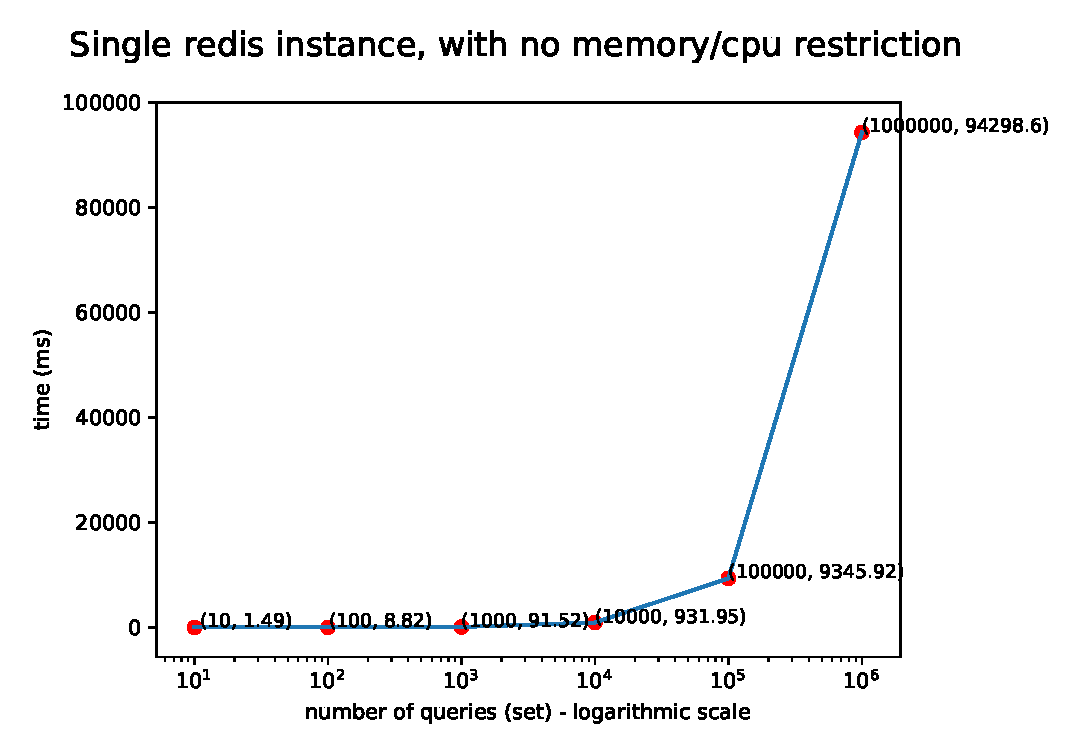
\includegraphics[width=\textwidth]{fig1.eps}
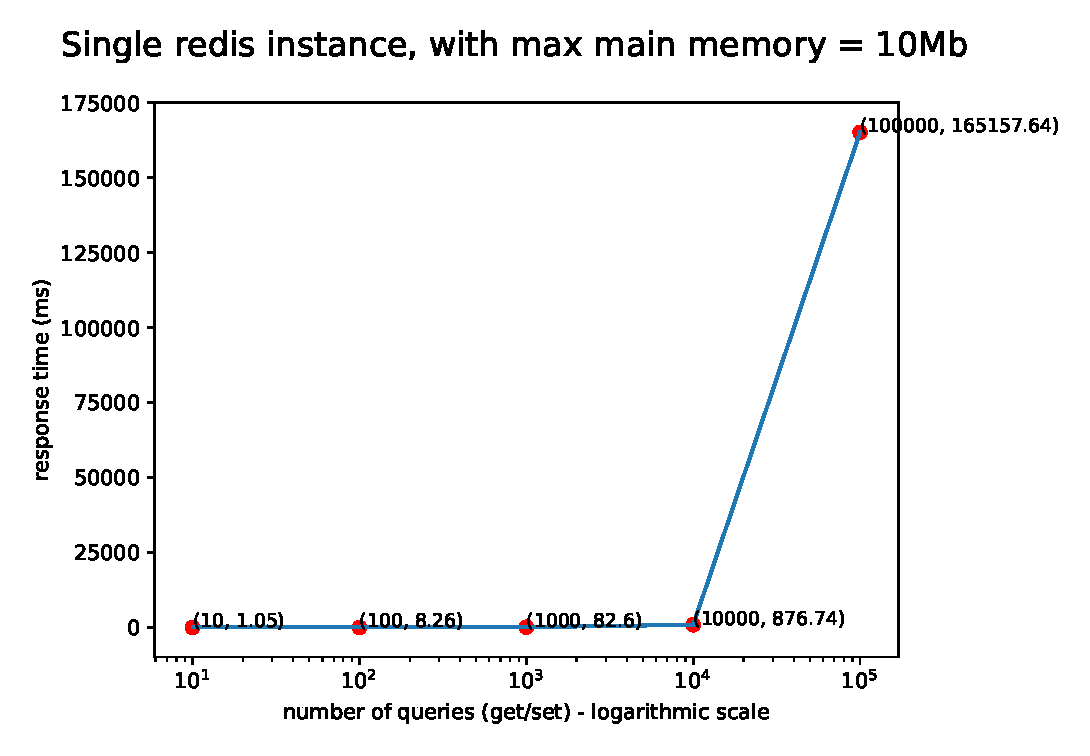
\includegraphics[width=\textwidth]{fig2.eps}
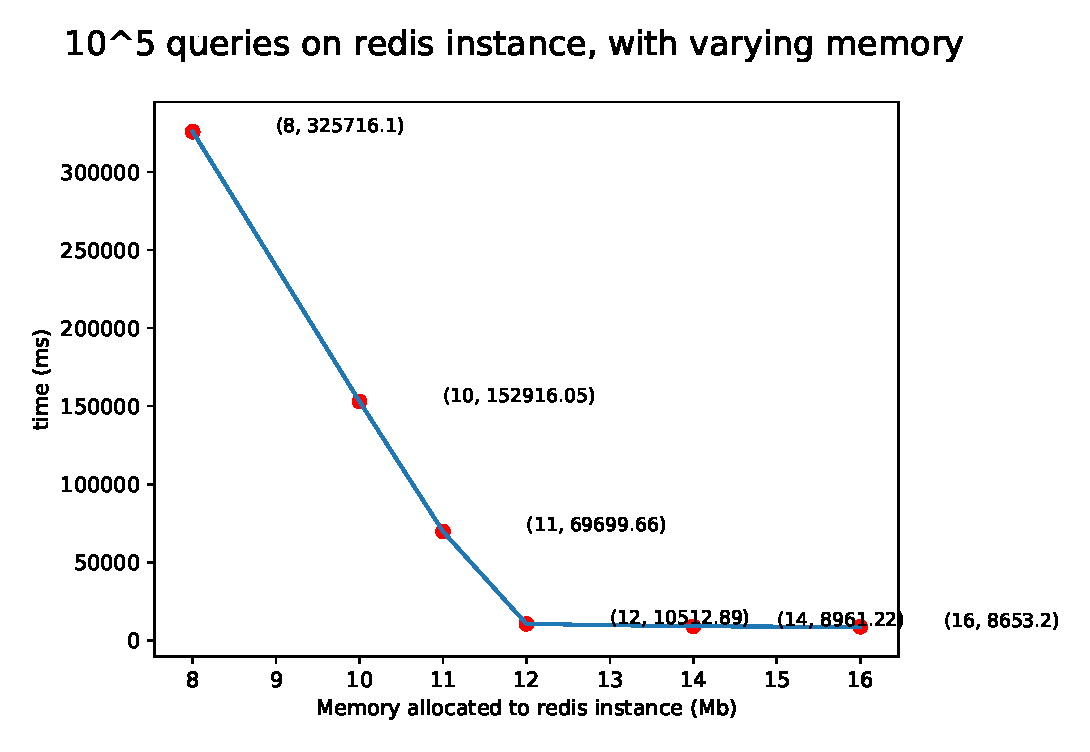
\includegraphics[width=\textwidth]{fig3.eps}
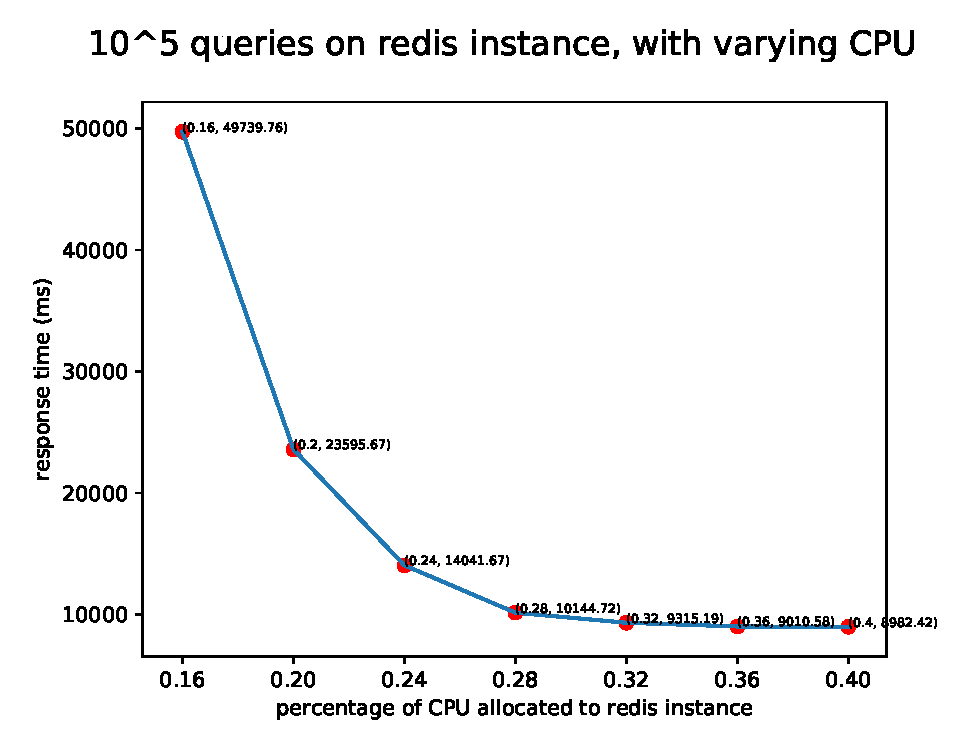
\includegraphics[width=\textwidth]{fig4.eps}






\pagebreak
\begin{thebibliography}{9}

\bibitem{redis}
Redis documentation,
\texttt{redis.io}
        
\bibitem{scaling}
Bondi, Andre.
\textit{Characteristics of scalability and their imapct on performace.}
WOSP, 2000.

\bibitem{twem}
Twemproxy, developed by twitter,
\texttt{github.com/twitter/twemproxy}

\end{thebibliography}

\end{document}
